\documentclass[journal,12pt,twocolumn]{IEEEtran}

\usepackage{setspace}
\usepackage{gensymb}
\singlespacing
\usepackage[cmex10]{amsmath}
\usepackage{amssymb}
\usepackage{xurl}

\usepackage{amsthm}
\usepackage{comment}
\usepackage{mathrsfs}
\usepackage{txfonts}
\usepackage{stfloats}
\usepackage{bm}
\usepackage{cite}
\usepackage{cases}
\usepackage{subfig}

\usepackage{longtable}
\usepackage{multirow}
\usepackage{float}
\usepackage{enumitem}
\usepackage{mathtools}
\usepackage{steinmetz}
\usepackage{tikz}
\usepackage{circuitikz}
\usepackage{verbatim}
\usepackage{tfrupee}
\usepackage[breaklinks=true]{hyperref}
\usepackage{graphicx}
\usepackage{tkz-euclide}

\usetikzlibrary{calc,math}
\usepackage{listings}
    \usepackage{color}                                            %%
    \usepackage{array}                                            %%
    \usepackage{longtable}                                        %%
    \usepackage{calc}                                             %%
    \usepackage{multirow}                                         %%
    \usepackage{hhline}                                           %%
    \usepackage{ifthen}                                           %%
    \usepackage{lscape}     
\usepackage{multicol}
\usepackage{chngcntr}

\DeclareMathOperator*{\Res}{Res}

\renewcommand\thesection{\arabic{section}}
\renewcommand\thesubsection{\thesection.\arabic{subsection}}
\renewcommand\thesubsubsection{\thesubsection.\arabic{subsubsection}}

\renewcommand\thesectiondis{\arabic{section}}
\renewcommand\thesubsectiondis{\thesectiondis.\arabic{subsection}}
\renewcommand\thesubsubsectiondis{\thesubsectiondis.\arabic{subsubsection}}


\hyphenation{op-tical net-works semi-conduc-tor}
\def\inputGnumericTable{}                                 %%

\lstset{
%language=C,
frame=single, 
breaklines=true,
columns=fullflexible
}
\begin{document}


\newtheorem{theorem}{Theorem}[section]
\newtheorem{problem}{Problem}
\newtheorem{proposition}{Proposition}[section]
\newtheorem{lemma}{Lemma}[section]
\newtheorem{corollary}[theorem]{Corollary}
\newtheorem{example}{Example}[section]
\newtheorem{definition}[problem]{Definition}

\newcommand{\BEQA}{\begin{eqnarray}}
\newcommand{\EEQA}{\end{eqnarray}}
\newcommand{\define}{\stackrel{\triangle}{=}}
\bibliographystyle{IEEEtran}
\raggedbottom
\setlength{\parindent}{0pt}
\providecommand{\mbf}{\mathbf}
\providecommand{\pr}[1]{\ensuremath{\Pr\left(#1\right)}}
\providecommand{\qfunc}[1]{\ensuremath{Q\left(#1\right)}}
\providecommand{\sbrak}[1]{\ensuremath{{}\left[#1\right]}}
\providecommand{\lsbrak}[1]{\ensuremath{{}\left[#1\right.}}
\providecommand{\rsbrak}[1]{\ensuremath{{}\left.#1\right]}}
\providecommand{\brak}[1]{\ensuremath{\left(#1\right)}}
\providecommand{\lbrak}[1]{\ensuremath{\left(#1\right.}}
\providecommand{\rbrak}[1]{\ensuremath{\left.#1\right)}}
\providecommand{\cbrak}[1]{\ensuremath{\left\{#1\right\}}}
\providecommand{\lcbrak}[1]{\ensuremath{\left\{#1\right.}}
\providecommand{\rcbrak}[1]{\ensuremath{\left.#1\right\}}}
\theoremstyle{remark}
\newtheorem{rem}{Remark}
\newcommand{\sgn}{\mathop{\mathrm{sgn}}}
\providecommand{\abs}[1]{\vert#1\vert}
\providecommand{\res}[1]{\Res\displaylimits_{#1}} 
\providecommand{\norm}[1]{\lVert#1\rVert}
%\providecommand{\norm}[1]{\lVert#1\rVert}
\providecommand{\mtx}[1]{\mathbf{#1}}
\providecommand{\mean}[1]{E[ #1 ]}
\providecommand{\fourier}{\overset{\mathcal{F}}{ \rightleftharpoons}}
%\providecommand{\hilbert}{\overset{\mathcal{H}}{ \rightleftharpoons}}
\providecommand{\system}{\overset{\mathcal{H}}{ \longleftrightarrow}}
	%\newcommand{\solution}[2]{\textbf{Solution:}{#1}}
\newcommand{\solution}{\noindent \textbf{Solution: }}
\newcommand{\cosec}{\,\text{cosec}\,}
\providecommand{\dec}[2]{\ensuremath{\overset{#1}{\underset{#2}{\gtrless}}}}
\newcommand{\myvec}[1]{\ensuremath{\begin{pmatrix}#1\end{pmatrix}}}
\newcommand{\mydet}[1]{\ensuremath{\begin{vmatrix}#1\end{vmatrix}}}
\numberwithin{equation}{subsection}
\makeatletter
\@addtoreset{figure}{problem}
\makeatother
\let\StandardTheFigure\thefigure
\let\vec\mathbf
\renewcommand{\thefigure}{\theproblem}
\def\putbox#1#2#3{\makebox[0in][l]{\makebox[#1][l]{}\raisebox{\baselineskip}[0in][0in]{\raisebox{#2}[0in][0in]{#3}}}}
     \def\rightbox#1{\makebox[0in][r]{#1}}
     \def\centbox#1{\makebox[0in]{#1}}
     \def\topbox#1{\raisebox{-\baselineskip}[0in][0in]{#1}}
     \def\midbox#1{\raisebox{-0.5\baselineskip}[0in][0in]{#1}}
\vspace{3cm}
\title{ Assignment 3}
\author{Savarana Datta - AI20BTECH11008}
\maketitle
\newpage
\bigskip
\renewcommand{\thefigure}{\theenumi}
\renewcommand{\thetable}{\theenumi}
Download all python codes from 
\begin{lstlisting}
https://github.com/SavaranaDatta/EE3900/tree/main/Assignment3/codes
\end{lstlisting}
%
and latex codes from 
%
\begin{lstlisting}
https://github.com/SavaranaDatta/EE3900/tree/main/Assignment3/Assignment3.tex
\end{lstlisting}


\section{Construction 2.16}
Let ABC be a right triangle in which a=8 , c=6 and $\angle B = 90 \degree$. BD is the perpendicular from $\vec{B}$ on AC (altitude). The circle through $\vec{B},\vec{C},\vec{D}$( circumcircle of $\Delta$BCD ) is drawn. Construct the tangents from $\vec{A}$ to this circle.

\section{Solution}
\begin{lemma}
If $\Delta ABC$ is a right angled triangle at $\vec{B}(\text{Be } \vec{O})$, then the points of contact of tangents from $\vec{A}$ to the circumcircle of $\Delta BCD$ (where $\vec{D}$ is the foot of perpendicular from $\vec{B}$ to side AC) are $\vec{B}$ and $\vec{P}$
\begin{align}
  \vec{P}&=2\vec{A}+2\lambda \brak{\frac{\vec{C}}{2}-\vec{A}}\\
  \text{where  } \lambda &= \frac{a^2}{a^{2}+\frac{c^{2}}{4}}
\end{align}
\end{lemma}
\begin{proof}
Given,\\
$\Delta ABC$ is a right angled triangle at $\vec{B}$(be $\vec{O}$) and $\vec{D}$ is the foot of perpendicular from $\vec{B}$ to the side AC.\\
As $\Delta BCD$ is right angled at $\vec{D}$, the circumcentre($\vec{C_{1}}$) is the midpoint of side BC and radius(r) is half the length of BC
\begin{align}
    \vec{C_{1}}&=\frac{\vec{B}+\vec{C}}{2}\\
    \implies \vec{C_1}& = \frac{\vec{C}}{2}\\
    r&=\frac{a}{2}
\end{align}
As $\Delta ABC$ is right angled at $\vec{B}$
\begin{align}
\brak{\vec{A}-\vec{B}}^\top\brak{\vec{C}-\vec{B}}&=0\\
\implies \vec{A}^{\top}\vec{C}&=0
\label{eq1}
\end{align}
 $\vec{B}$ is one of the points of contact of tangent to the circle.
\begin{figure}[!ht]
   \centering
   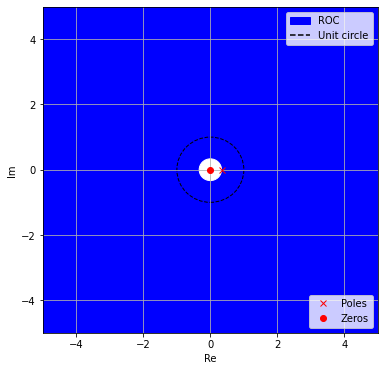
\includegraphics[width=\columnwidth]{fig1.png}
   \caption{Reference plot}
\end{figure}
Let $\vec{M}$ be the point of intersection of BP and A$C_1$\\
As $\vec{M}$ lies on the line A$C_{1}$
\begin{align}
    \vec{M}=\vec{A}+\lambda\brak{\frac{\vec{C}}{2}-\vec{A}}
\end{align}
As BM is perpendicular to A$C_1$
\begin{align}
    \brak{\vec{M}-\vec{B}}^\top \brak{\frac{\vec{C}}{2}-\vec{A}} &=0\\
    \brak{\vec{A}+\lambda\brak{\frac{\vec{C}}{2}-\vec{A}}}^\top\brak{\frac{\vec{C}}{2}-\vec{A}}&=0\\
    \vec{A}^\top\frac{\vec{C}}{2}-\vec{A}^\top\vec{A}+\lambda\brak{\norm{\frac{\vec{C}}{2}-\vec{A}}^2}&=0\\
    \lambda=\frac{\vec{A}^\top\vec{A}-\vec{A}^\top\frac{\vec{C}}{2}}{\norm{\frac{\vec{C}}{2}-\vec{A}}^2}
\end{align}
From \ref{eq1} we have
\begin{align}
    \lambda=\frac{a^{2}}{a^{2}+\frac{c^{2}}{4}}
\end{align}
As $\vec{M}$ is midpoint of $\vec{B}$ and $\vec{P}$
\begin{align}
    \vec{M}&=\frac{\vec{B}+\vec{P}}{2}\\
    \implies
    \vec{P}&=2\vec{M}\\
    \implies \vec{P}&=2\brak{\vec{A}+\lambda\brak{\frac{\vec{C}}{2}-\vec{A}}}
\end{align}

\end{proof}
Let
\begin{align}
    \vec{B}=\myvec{0\\0}\\
    \implies \vec{C}=\myvec{8\\0} \\
    \implies  \vec{A}=\myvec{0\\6}
\end{align}
The centre and the radius of circumcircle is given by 
\begin{align}
    \vec{C_1}=\myvec{4\\0}\\
    r = \frac{a}{2}=4
\end{align}
The equation of circumcircle of $\Delta BCD$ is 
\begin{align}
    \vec{x}^\top\vec{x}-2\vec{C_1}\vec{x}+f &=0\\
    \implies \vec{x}^\top\vec{x}-\myvec{8&0}\vec{x}&=0
    \label{eq4}
\end{align}
\begin{figure}[!ht]
   \centering
   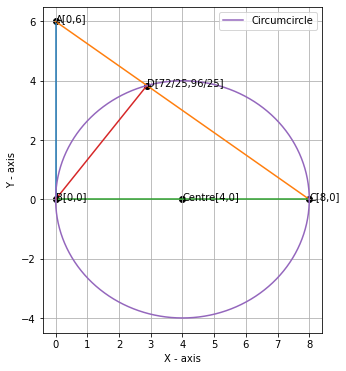
\includegraphics[width=\columnwidth]{fig2.png}
   \caption{The plot of circumcircle of $\Delta BCD$}
\end{figure}
from the above lemma, points of contact of tangents from $\vec{A}$ are
\begin{align}
    \vec{B}&=\myvec{0\\0} \text{  and}\\
    \vec{P}&=2\vec{A}+2\lambda\brak{\frac{\vec{C}}{2}-\vec{A}}\\
   \implies \vec{P}&=\myvec{\frac{72}{13}\\ \frac{48}{13}}
\end{align}
Equation of tangent 1 (AB)
\begin{align}
    \vec{x}&=\vec{B}+\lambda\vec{m}\\
    \vec{x}&=\lambda\myvec{0\\1}
\end{align}
Equation of tangent 2 (AP)
\begin{align}
    \vec{x}&=\vec{A}+\lambda\vec{m}\\
    \vec{x}&=\myvec{0\\6}+\lambda\brak{\myvec{0\\6}-\myvec{\frac{72}{13}\\ \frac{48}{13}}}\\
    \vec{x}&=\myvec{0\\6}+\lambda\myvec{1\\ \frac{-5}{12}}
\end{align}
\begin{figure}[!ht]
   \centering
   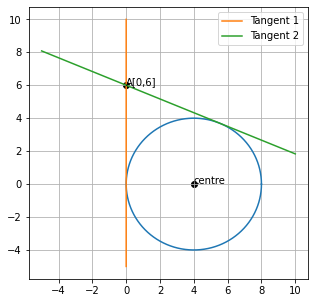
\includegraphics[width=\columnwidth]{fig3.png}
   \caption{The plot of tangents}
\end{figure}
\end{document}